\usecolorstyle{TitleStyle}
\block[bodyinnersep=0em]{How improve PINN prediction ? \textnormal{\Large - Using enriched FEM}}{}
\usecolorstyle{myColorStyle}

\begin{columns}

    \column{0.5}

    \block{Additive approach}{
        \vspace{-20pt}
        \begin{center}
            \begin{tcolorbox}[
                colback=color1!50, % Couleur de fond de la boîte
                colframe=color2, % Couleur du cadre de la boîte
                arc=2mm, % Rayon de l'arrondi des coins
                boxrule=2pt, % Épaisseur du cadre de la boîte
                breakable, enhanced jigsaw,
                width=\linewidth
                ]       
                % \begin{minipage}{0.77\linewidth}     
                The enriched approximation space is defined by
                \begin{equation*}
                    V_h^+ = \left\{u_h^+=u_\theta+p_h^+ \;, \; p_h^+ \in V_h^0\right\}
                \end{equation*}

                with $V_h^0$ the standard continuous Lagrange FE space and the weak problem becomes
                \begin{equation}
                    \label{eq:weakplus}
                    \text{Find } p_h^+ \in V_h^0, \; \forall v_h \in V_h^0,
                    \; a(p_h^+,v_h) = l(v_h) - a(u_{\theta},v_h),\tag{$\mathcal{P}_h^+$}
                \end{equation}
                
                \vspace{5pt}
                with modified boundary conditions and
                \begin{equation*}
                    a(u,v)=\int_{\Omega} \nabla u \cdot \nabla v, \quad l(v)=\int_{\Omega} f \, v.
                \end{equation*}
                    % \textbf{General Dirichlet BC :} $\quad p_h^+ = - u_{\theta} \;\text{on}\; \Gamma$.
                % \end{minipage} \;
                % \begin{minipage}{0.2\linewidth} 
                    % \centering
                    % \includegraphics[width=\linewidth]{images/corr/correction2.pdf}
                % \end{minipage}
                
                \centering
                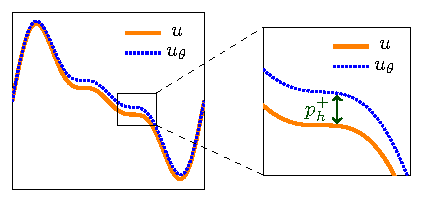
\includegraphics[width=0.8\linewidth]{images/corr/correction.pdf}
            \end{tcolorbox}
        \end{center}
        \vspace{-30pt}
    }
    \block{Convergence analysis}{
        \vspace{-20pt}
        \begin{center}
            \begin{tcolorbox}[
                colback=color1!50, % Couleur de fond de la boîte
                colframe=color2, % Couleur du cadre de la boîte
                arc=2mm, % Rayon de l'arrondi des coins
                boxrule=2pt, % Épaisseur du cadre de la boîte
                breakable, enhanced jigsaw,
                width=\linewidth
                ]            
                Considering $u$ as the solution of the Poisson problem and $u_{\theta}$ as the PINN prediction.

                \hypersetup{citecolor=white}

                \begin{center}
                    \begin{mytheo}{Convergence analysis of the standard FEM \cite{Ern2004TheoryAP}}{fem}
                        We denote $u_h\in V_h^0$ the discrete solution of standard FEM with $V_h^0$ a $\mathbb{P}_k$ Lagrange space. Thus,
                        \vspace{-5pt}
                        \begin{equation*}
                            | u-u_h|_{H^1} \le C_{H^1} \, h^{k} |u|_{H^{k+1}},
                        \end{equation*}
                        \begin{equation*}
                            \| u-u_h\|_{L^2} \le C_{L^2} \, h^{k+1} |u|_{H^{k+1}}.
                        \end{equation*}
                    \end{mytheo}

                    \begin{mytheo}{Convergence analysis of the enriched FEM \cite{ours_2024}}{add}
                        We denote $u_h^+\in V_h^+$ the discrete solution of (\ref{eq:weakplus}) with $V_h^+$ a $\mathbb{P}_k$ Lagrange space. Thus
                        % \hspace{485pt} \begin{minipage}{0.2\linewidth}
                        %     \large \textbf{\textcolor{orange}{$C_{\text{gain}}$}}
                        % \end{minipage}
                        \begin{equation*}
                            | u-u_h^+|_{H^1} \le \fcolorbox{orange}{color1!30}{$\frac{| u-u_{\theta} |_{H^{k+1}}}{| u |_{H^{k+1}}}$} \left(C_{H^1} \, h^{k} |u|_{H^{k+1}}\right),
                        \end{equation*}
                        and
                        \begin{equation*}
                            \| u-u_h^+\|_{L^2} \le \fcolorbox{orange}{color1!30}{$\frac{| u-u_{\theta} |_{H^{k+1}}}{| u |_{H^{k+1}}}$} \left(C_{L^2} \, h^{k+1} |u|_{H^{k+1}}\right).
                        \end{equation*}
                    \end{mytheo}
                \end{center}
                
                \textcolor{orange}{Theoretical gain of the additive approach.}

                \hypersetup{citecolor=color2}

                % \textit{Remark :} The constant $C_{\text{gain}}$ shows that the closer the prior is to the solution, the lower the error constant associated with the method.
            \end{tcolorbox}
        \end{center}	
        \vspace{-30pt}
    }

    
    \usecolorstyle{myColorStyle}
    \useblockstyle{TornOut}
    
    \column{0.5}
    
    \block{Problem considered \textnormal{- Numerical results}}{
        \vspace{-20pt}
        \begin{tcolorbox}[
            colback=color1!50, % Couleur de fond de la boîte
            colframe=color2, % Couleur du cadre de la boîte
            arc=2mm, % Rayon de l'arrondi des coins
            boxrule=2pt, % Épaisseur du cadre de la boîte
            breakable, enhanced jigsaw,
            width=\linewidth
            ]            
            \ding{217} Spatial domain : $\Omega=[-0.5\pi,0.5\pi]^2$ \\
            \ding{217} Parametric domain : $\mathcal{M}=[-0.5,0.5]^2$ \\
            \ding{217} Analytical solution :               
            \vspace{-20pt}
            \begin{equation*}
                u_{ex}\big((x,y),\mu\big)=\exp\left(-\frac{(x-\mu_1)^2+(y-\mu_2)^2}{2}\right)\sin(2x)\sin(2y)
            \end{equation*} 
            with $\mu=(\mu_1,\mu_2)\in\mathcal{M}$ (\textbf{\fcolorbox{color1!50}{color1}{parametric}}) and the associated source term $f$.
        \end{tcolorbox}
        \vspace{-30pt}
    }

    \block{Numerical results \textnormal{- Improve errors}}{
        \vspace{-20pt}
        \begin{minipage}{0.49\linewidth}
            \centering
            \begin{tcolorbox}[
                colback=color1!50, % Couleur de fond de la boîte
                colframe=color2, % Couleur du cadre de la boîte
                arc=2mm, % Rayon de l'arrondi des coins
                boxrule=2pt, % Épaisseur du cadre de la boîte
                breakable, enhanced jigsaw,
                width=\linewidth
                ]     
                \textbf{Error estimates :} $\mu=(0.05, 0.22)$.
                
                \vspace{-10pt}
                \hspace{-50pt}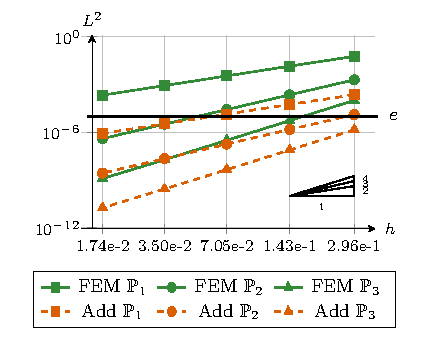
\includegraphics[width=1.18\linewidth]{images/numeric/poisson/dirichlet/cvg/cvg.pdf}
                % \normalsize
                % \textit{Remark :} We note N the number of nodes in each direction of the square \big(Total : $N^2$\big).
            \end{tcolorbox}
        \end{minipage} \;
        \begin{minipage}{0.49\linewidth}
            \centering
            \begin{tcolorbox}[
                colback=color1!50, % Couleur de fond de la boîte
                colframe=color2, % Couleur du cadre de la boîte
                arc=2mm, % Rayon de l'arrondi des coins
                boxrule=2pt, % Épaisseur du cadre de la boîte
                breakable, enhanced jigsaw,
                width=\linewidth
                ]            
                \textbf{Gains achieved :} $50$ sets of parameters.
                $$S=\left\{\mu^{(1)},\dots,\mu^{(50)}\right\}$$
                
                \vspace{5pt}
                \centering
                \fcolorbox{white}{white}{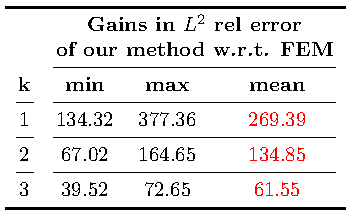
\includegraphics[width=\linewidth]{images/numeric/poisson/dirichlet/gains/gains.pdf}}

                \vspace{5pt}
                Gain : $\| u-u_h\|_{L^2} / \| u-u_h^+\|_{L^2}$ \\
                
                \vspace{10pt}
                Cartesian mesh : $20^2$ nodes.
                \vspace{8pt}
            \end{tcolorbox}
        \end{minipage}
        \vspace{-20pt}
    }

    \block{Numerical results \textnormal{- Improve numerical costs}}{
        \vspace{-30pt}
        \begin{center}
            \begin{tcolorbox}[
                colback=color1!50, % Couleur de fond de la boîte
                colframe=color2, % Couleur du cadre de la boîte
                arc=2mm, % Rayon de l'arrondi des coins
                boxrule=2pt, % Épaisseur du cadre de la boîte
                breakable, enhanced jigsaw,
                width=\linewidth
                ]       
                
                \textbf{$N_\text{dofs}$ required to reach the same error $e$ :} $\mu=(0.05, 0.22)$.
                
                \vspace{20pt}
                \begin{minipage}{0.49\linewidth}
                    \flushright
                    \fcolorbox{white}{white}{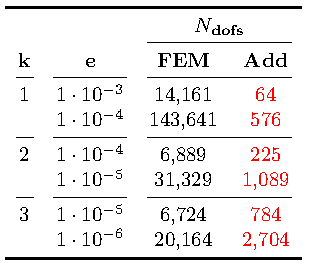
\includegraphics[width=0.7\linewidth]{images/numeric/poisson/dirichlet/costs/costs.pdf}}
                \end{minipage}
                \begin{minipage}{0.49\linewidth}
                    \flushleft \quad
                    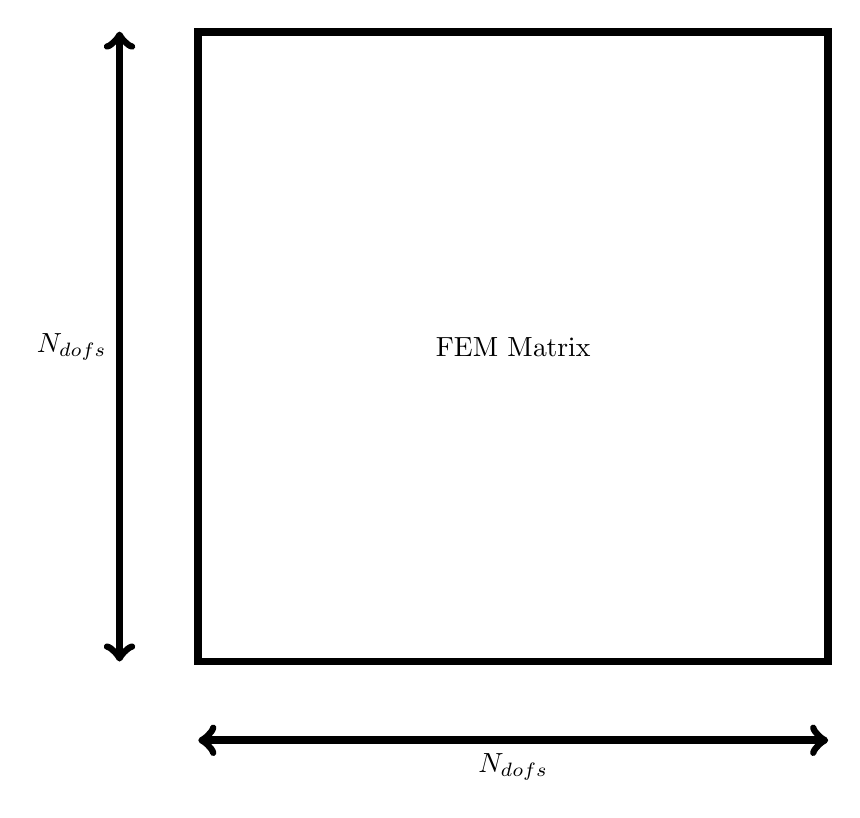
\begin{tikzpicture}

                        % Dessin de la matrice (grille)
                        \draw[line width=1mm, black] (0,0) rectangle (8,8); % Contour

                        % Add text with "FEM Matrix" in the center 
                        \node at (4,4) {FEM Matrix};

                        % \foreach \x in {1,2,3,4,5} {
                        %     \draw[black] (\x,0) -- (\x,8);
                        %     \draw[black] (0,\x) -- (8,\x);
                        % }
                        
                        % Flèche horizontale en dessous
                        \draw[line width=1mm, <->] (0,-1) -- (8,-1) node[midway, below] {$N_{\text{dofs}}$};
                        
                        % Flèche verticale à gauche
                        \draw[line width=1mm, <->] (-1,0) -- (-1,8) node[midway, left] {$N_{\text{dofs}}$};
                    
                    \end{tikzpicture}
                \end{minipage}

                \centering
                Less degrees of freedom  $\quad\Rightarrow \quad \left\{\begin{aligned}
                    &\;\text{Lower numerical cost} \\
                    &\;\text{Faster simulation}
                \end{aligned}\right.$ 
            \end{tcolorbox}
        \end{center}
        \vspace{-30pt}
    }

    % \usecolorstyle{bibStyle}
    % \useblockstyle{Default}

	% \block{
	% 	\vspace{-40pt}
	% 	\footnotesize
	% 	\printbibliography[heading=none]
	% }

\end{columns}